% Copyright 2004 by Till Tantau <tantau@users.sourceforge.net>.
%
% In principle, this file can be redistributed and/or modified under
% the terms of the GNU Public License, version 2.
%
% However, this file is supposed to be a template to be modified
% for your own needs. For this reason, if you use this file as a
% template and not specifically distribute it as part of a another
% package/program, I grant the extra permission to freely copy and
% modify this file as you see fit and even to delete this copyright
% notice. 




\documentclass{beamer}

\usepackage[OT1]{fontenc}
\usepackage{polski}
\usepackage[utf8]{inputenc}
\usepackage{subfig}


% There are many different themes available for Beamer. A comprehensive
% list with examples is given here:
% http://deic.uab.es/~iblanes/beamer_gallery/index_by_theme.html
% You can uncomment the themes below if you would like to use a different
% one:
%\usetheme{AnnArbor}
%\usetheme{Antibes}
%\usetheme{Bergen}
%\usetheme{Berkeley}
%\usetheme{Berlin}
%\usetheme{Boadilla}
%\usetheme{boxes}
%\usetheme{CambridgeUS}
%\usetheme{Copenhagen}
%\usetheme{Darmstadt}
%\usetheme{default}
%\usetheme{Frankfurt}
%\usetheme{Goettingen}
%\usetheme{Hannover}
%\usetheme{Ilmenau}
%\usetheme{JuanLesPins}
%\usetheme{Luebeck}
\usetheme{Madrid}
%\usetheme{Malmoe}
%\usetheme{Marburg}
%\usetheme{Montpellier}
%\usetheme{PaloAlto}
%\usetheme{Pittsburgh}
%\usetheme{Rochester}
%\usetheme{Singapore}
%\usetheme{Szeged}
%\usetheme{Warsaw}

\beamertemplatenavigationsymbolsempty

\definecolor{ok}{RGB}{1, 115, 0}
\definecolor{nok}{RGB}{240, 191, 12}
\title[Sterowanie pozycyjne silnikami krokowymi.]{Sterowanie pozycyjne silnikami krokowymi}

% A subtitle is optional and this may be deleted
\subtitle{na przykładzie manipulatora dydaktycznego.}

\author{Michał Romanowski}
% - Give the names in the same order as the appear in the paper.
% - Use the \inst{?} command only if the authors have different
%   affiliation.

%\institute[Universities of Somewhere and Elsewhere] % (optional, but mostly needed)
%{
%  \inst{1}%
%  Department of Computer Science\\
%  University of Somewhere
%  \and
%  \inst{2}%
%  Department of Theoretical Philosophy\\
%  University of Elsewhere}
%% - Use the \inst command only if there are several affiliations.
%% - Keep it simple, no one is interested in your street address.

\date{2018}
% - Either use conference name or its abbreviation.
% - Not really informative to the audience, more for people (including
%   yourself) who are reading the slides online

%\subject{Theoretical Computer Science}
% This is only inserted into the PDF information catalog. Can be left
% out. 

% If you have a file called "university-logo-filename.xxx", where xxx
% is a graphic format that can be processed by latex or pdflatex,
% resp., then you can add a logo as follows:

% \pgfdeclareimage[height=0.5cm]{university-logo}{university-logo-filename}
% \logo{\pgfuseimage{university-logo}}

% Delete this, if you do not want the table of contents to pop up at
% the beginning of each subsection:
%\AtBeginSubsection[]
%{
%  \begin{frame}<beamer>{Outline}
%    \tableofcontents[currentsection,currentsubsection]
%  \end{frame}
%}

% Let's get started
\begin{document}

\begin{frame}
  \titlepage
\end{frame}

\begin{frame}{Plan prezentacji.}
  \tableofcontents
  % You might wish to add the option [pausesections]
\end{frame}

% Section and subsections will appear in the presentation overview
% and table of contents.
\section{Wstęp - manipulator dydaktyczny.}

\begin{frame}{Manipulator dydaktyczny.}
\begin{columns}[T]
	\begin{column}{.5\textwidth}
		\begin{itemize}
		\item {
			Projekt realizowany w ramach działalności koła naukowego KNR Bionik.
		}
		\item {
			Pierwszy prototyp powstał w semestrze 16Z.
		}
		\item {
			Aktualnie rozwijany jest drugi prototyp.	 	
		}
		\end{itemize}
	\end{column}
	\begin{column}{.5\textwidth}
		\begin{figure}%
			\centering
			\subfloat[Pierwszy prototyp]{{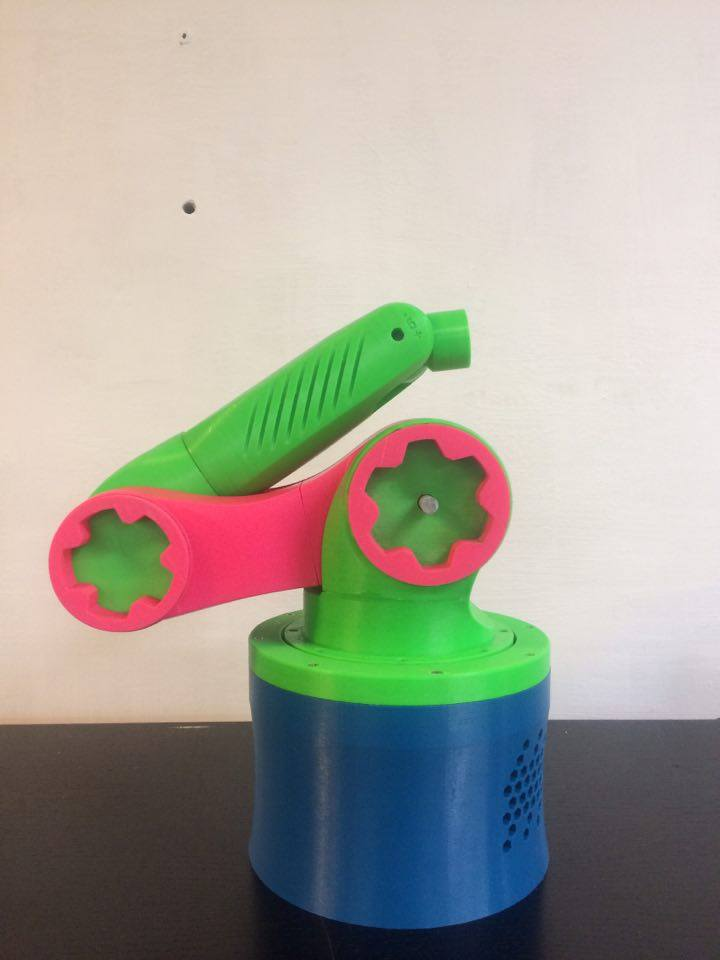
\includegraphics[width=.43\textwidth]{img/v1.png} }}%
			\qquad
			\subfloat[Aktualna wersja]{{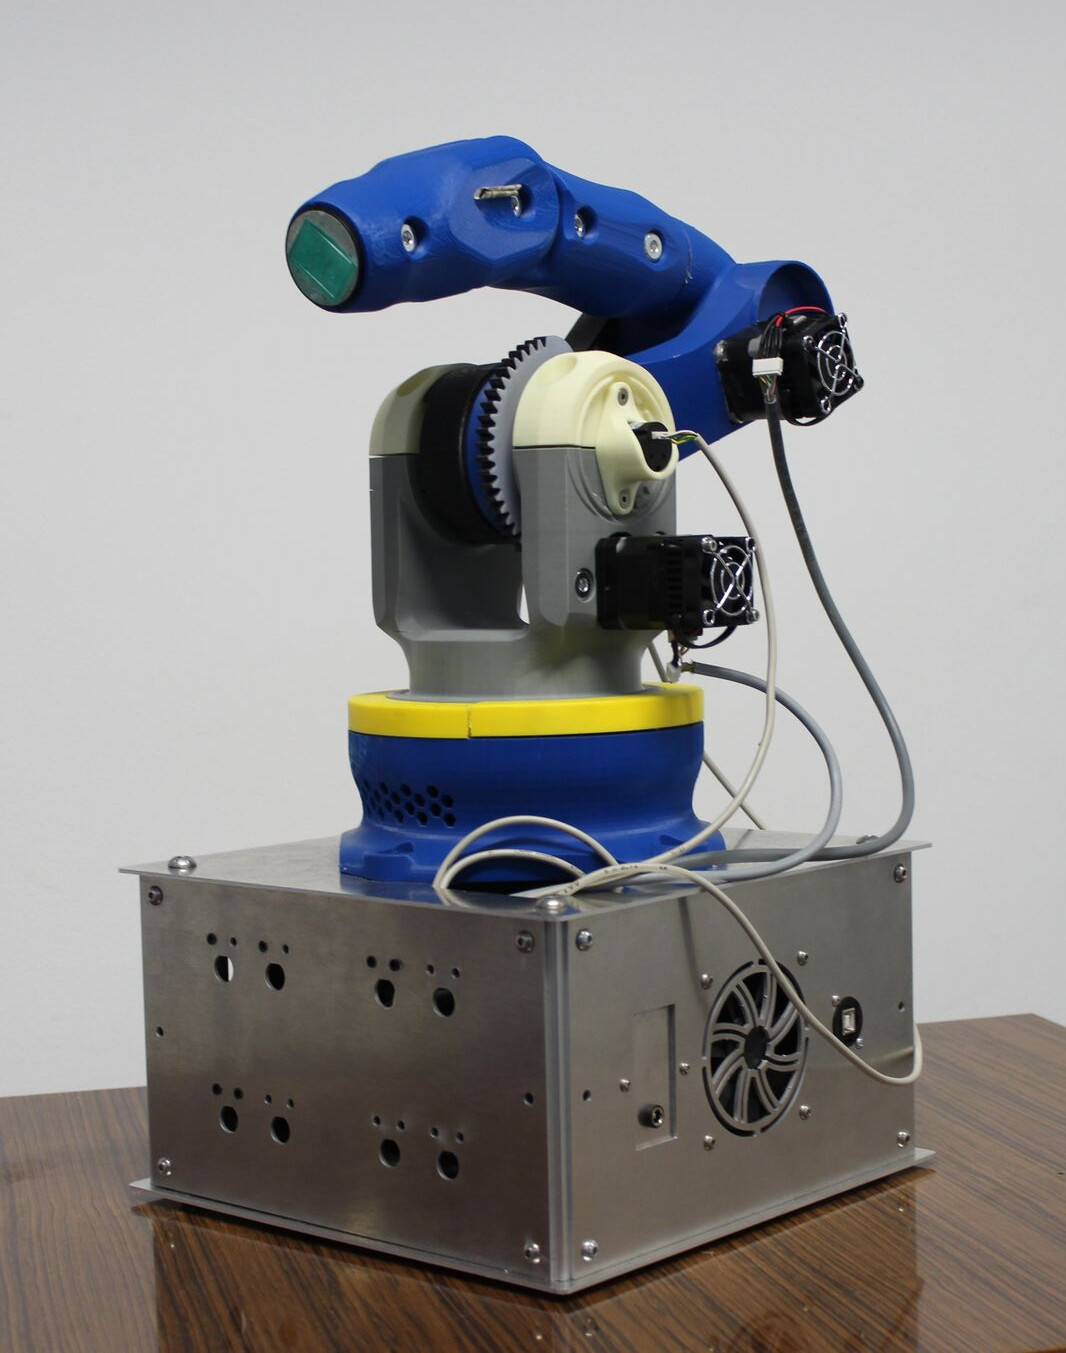
\includegraphics[width=.43\textwidth]{img/v2.jpeg} }}%
%			\caption{2 Figures side by side}%
			\label{fig:example}%
		\end{figure}
	\end{column}
\end{columns}
\end{frame}

\section{Struktura robota.}

\begin{frame}{Struktura robota.}
	\begin{itemize}
		\item {Trzy stopnie swobody.}
		\item {Enkodery na każdym stawie}.
		\item {System sterowania oparty na mikrokontrolerze \textit{STM32F411RE}.}
		\item {Sterownik silników krokowych oparty na układach \textit{Toshiba TB6560}.}
		\item {Zasilanie 12\textsc{V}.}
	\end{itemize}
\end{frame}

\section{Założenia projektu}
\begin{frame}{Założenia projektu.}

	\begin{itemize}
		\item {
			Sterowanie prędkościowe silnikami krokowymi.
		}
		\item {
			Zadawanie odpowiedniej trajektorii prędkości (w celu wyelminowania uderzenia).
		}
		\item {
			Sterowanie pozycyjne w pętli zamkniętej ze sprzężeniem od strony enkoderów.
		}
		\item{
			Ograniczenia na prędkości, przyśpieszenie, położenie.
		}
		\item{
			Komunikacja z komputerem.
		}
	\end{itemize}
		\begin{figure}%
			\centering
			\subfloat[Enkoder]{{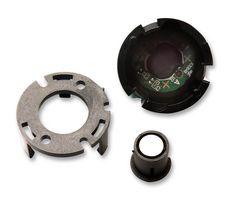
\includegraphics[width=.25\textwidth]{img/encoder_aeat6012_a06.jpg} }}%
			\qquad
			\subfloat[Sterownik silników krokowych]{{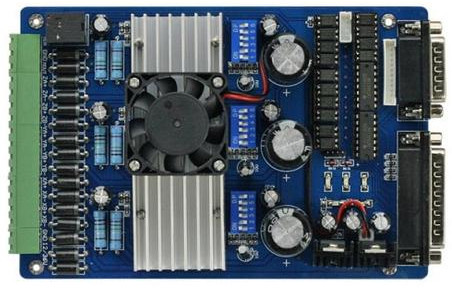
\includegraphics[width=.25\textwidth]{img/stepper_driver.jpg} }}%
			\qquad
			\subfloat[Silnik krokowy]{{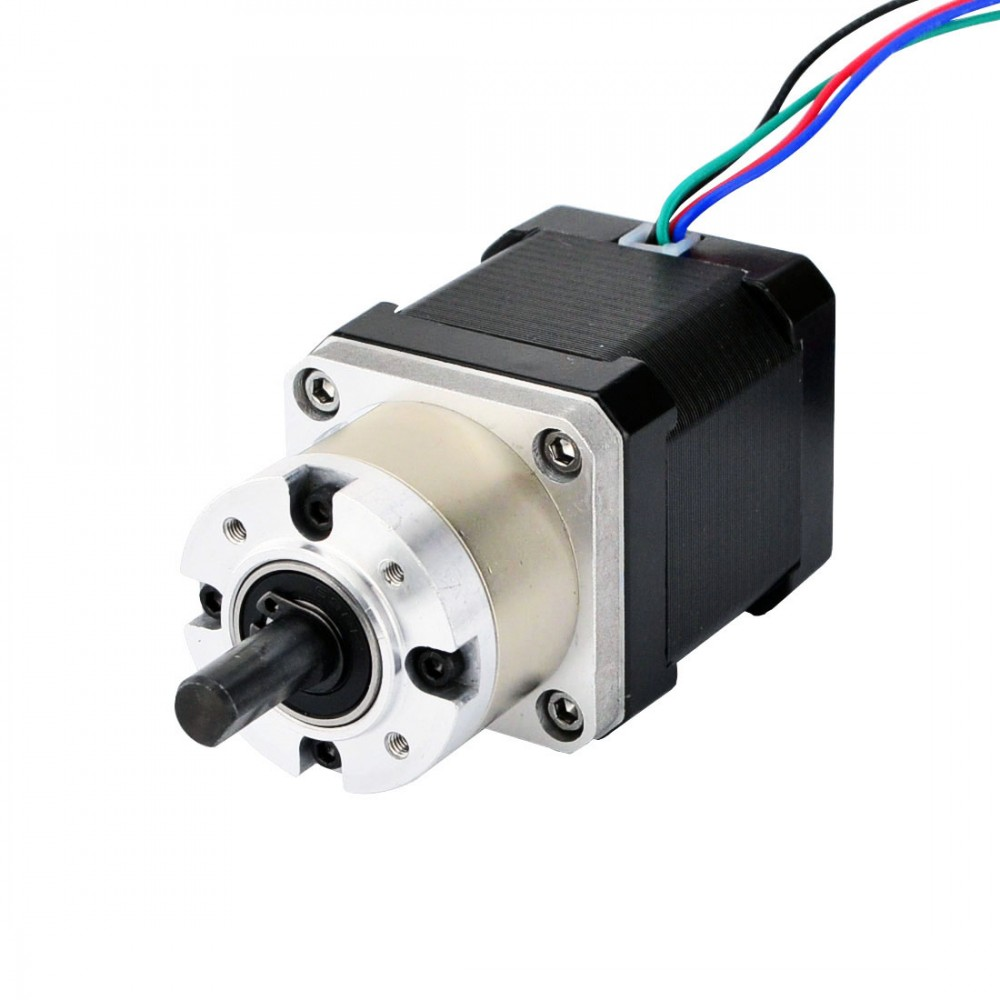
\includegraphics[width=.25\textwidth]{img/stepper_motor_gear.jpg} }}%
			\label{fig:example2}%
		\end{figure}
\end{frame}

\section{Aktualny stan prac.}
\begin{frame}{Aktualny stan prac.}
	\begin{columns}[T]
		\begin{column}{.5\textwidth}
			\textcolor{ok}{Wykonano:}
			\begin{itemize}
				\item Obsługa sterownika silników
				\item Obsługa enkoderów.
				\item Prędkościowe sterowanie silników
				\item Pozycyjne sterowanie silników w pętli zamkniętej.
			\end{itemize}
		\end{column}
		\begin{column}{.5\textwidth}
			\textcolor{nok}{W trakcie:}
			\begin{itemize}
				\item Ograniczenia na prędkości, przyśpieszenie, położenie.
				\item Komunikacja z komputerem.
				\item Tworzenie dokumentacji.
			\end{itemize}
		\end{column}
	\end{columns}
\end{frame}

\section{Lista współautorów.}
\begin{frame}{Lista współautorów.}
	
	\begin{columns}[T]
		\begin{column}{.5\textwidth}
			\begin{itemize}
				\item Hubert Kowalski 
				\item Kamil Foryszewski 
				\item Konrad Winnicki 
				\item Maciej Pawliński 
				\item Marcin Skrzypkowski 
				\item Marta Pacuszka 
				\item Michał Romanowski 
				\item Michał Stolarz 
				\item Piotr Matysiak 
				\item Tomasz Ziemnicki 
			\end{itemize}
		\end{column}
		\begin{column}{.5\textwidth}
			\begin{figure}
				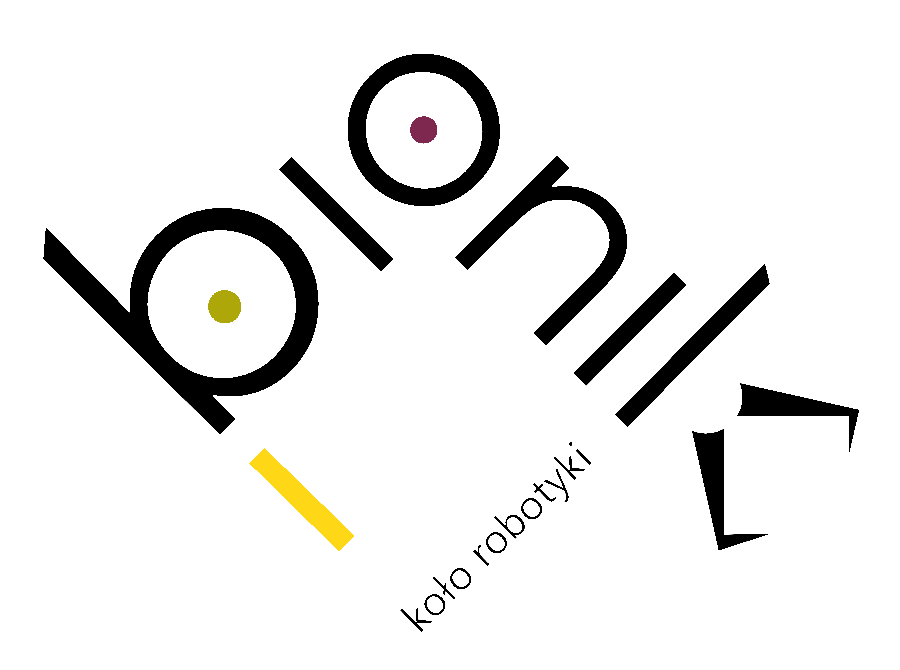
\includegraphics[width=1\textwidth]{img/logo.png}
			\end{figure}
		\end{column}
	\end{columns}
\end{frame}


\end{document}


